\documentclass{standalone}
\usepackage{tikz}

\begin{document}

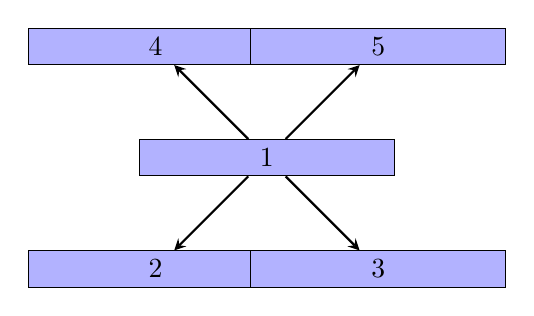
\begin{tikzpicture}[node distance=2cm, auto]
    % Define the style for the nodes
    \tikzset{
        topic/.style={rectangle, draw=black, fill=blue!30, text width=3cm, align=center},
        connector/.style={->, thick, >=stealth}
    }

    % Nodes
    \node[topic] (central) {1};
    \node[topic, below left of=central] (chapter2) {2};
    \node[topic, below right of=central] (chapter3) {3};
    \node[topic, above left of=central] (chapter4) {4};
    \node[topic, above right of=central] (chapter5) {5};

    % Edges
    \draw[connector] (central) -- (chapter2);
    \draw[connector] (central) -- (chapter3);
    \draw[connector] (central) -- (chapter4);
    \draw[connector] (central) -- (chapter5);

    % Optional: Add labels or descriptions if needed
    % \node at (central.west) [anchor=east] {Central Topic};
    % \node at (chapter2.south west) [anchor=north east] {Chapter 2};
    % \node at (chapter3.south east) [anchor=north west] {Chapter 3};
    % \node at (chapter4.north west) [anchor=south east] {Chapter 4};
    % \node at (chapter5.north east) [anchor=south west] {Chapter 5};
\end{tikzpicture}

\end{document}